El presente capítulo aborda la concepción teórica y práctica del diseño de \textit{Reset}. Dado que las vertientes narrativa, referencial y estética han supuesto pilares de diseño críticos desde la génesis del proyecto, esta sección formaliza las directrices conceptuales y creativas de la obra. A lo largo de las secciones consecutivas, se detalla el trasfondo argumental y el guion, el diseño de niveles (\textit{Level Design}), el sistema de interfaces de usuario (UI/UX), la coherencia visual basada en el estilo Pixel Art y las referencias culturales y artísticas a títulos de la industria que guían y justifican el posterior desarrollo técnico del videojuego.

% =========================================================================
\section{Historia de Reset}
\subsection{Concepto y contexto narrativo}
\label{subsec:concepto}

La premisa conceptual y narrativa de \textit{Reset} se sitúa en el interior de una consola de videojuegos clásica que lleva años acumulando polvo, abandonada en el rincón de una habitación. Por fuera, el hardware luce apagado, inerte y frío; un electrodoméstico obsoleto que permanece enchufado pero ignorado por su dueño. Sin embargo, en su interior late una realidad completamente distinta: los mundos digitales de los cartuchos y los datos almacenados siguen vivos y activos bajo la penumbra del circuito integrado. Sus personajes continúan existiendo en una vigilia eterna, ajenos al olvido exterior y creyendo que sus respectivos mundos representan la única y absoluta realidad.

No obstante, el paso del tiempo y la falta de uso han comenzado a pasar factura al sistema. El polvo se ha infiltrado en los chips de memoria y los condensadores empiezan a fallar debido al envejecimiento físico de los componentes del hardware. La propia unidad de procesamiento central de la consola (la CPU) es de las pocas conscientes de esta lenta agonía: detecta los sectores corruptos y sabe que, si se apaga de forma definitiva, toda la información, los mundos y las vidas que alberga se borrarán para siempre en un olvido digital absoluto. En un intento desesperado por sobrevivir, la consola planea un reinicio global (\textit{Reset}) para purgar los errores y canalizar la energía suficiente para encender su pantalla exterior una vez más. Su objetivo final tiene un tinte melancólico y esperanzador: enviar una señal física al mundo exterior, encendiendo sus luces y emitiendo sonido, con la esperanza de llamar la atención de su antiguo dueño, reavivar su curiosidad infantil por jugar y salvar el sistema antes de que sea demasiado tarde.

Para llevar a cabo este reinicio, la consola necesita recuperar los núcleos operativos de sus diferentes videojuegos, pero el sistema no posee la capacidad de interactuar directamente en las simulaciones; requiere un agente activo que juegue y complete los niveles desde dentro. Para esta tarea, la consola toma una decisión lógica pero inusual: selecciona a un NPC (\textit{Non-Player Character}) genérico, el avatar del tutorial de uno de sus juegos. Al no tener un nombre, una personalidad predefinida ni un rol heroico asignado en su código, y teniendo en cuenta su propósito original de enseñar al jugador, este personaje resulta ser la página en blanco ideal para aprender y dominar las diversas mecánicas de todos los géneros que habitan el sistema, sin saber que dentro de sí mismo posee una habilidad increíble de aprendizaje, asimilación y captación de mecánicas de juego heterogéneas.

\subsection{Historia del prototipo jugable}
\label{subsec:historia}

El juego comienza cuando el protagonista despierta confuso y temeroso en el \textbf{Hub (el Nexo)}. Este lugar, que en los años dorados de la consola era una bulliciosa oficina central donde innumerables procesos y subrutinas trabajaban en armonía para que el sistema funcionase, se muestra ahora como una terminal vacía, silenciosa y fantasmal. Allí, la consola interactúa con el protagonista. A través de un diálogo directo, le revela la cruda realidad: que su mundo es una simulación dentro de una máquina moribunda y que él es el único capaz de cruzar los portales de los juegos para recuperar los núcleos y salvar su existencia colectiva. Esto se debe a que todos los demás personajes de la consola siguen viviendo en sus respectivos mundos digitales pensando que son realidades absolutas, ignorando por completo la inminente destrucción de la máquina. El protagonista, encarnando el inicio del viaje del héroe clásico, experimenta miedo y confusión, pero la inminencia del colapso no le deja otra opción que aceptar la misión.

A medida que el protagonista avanza por los mundos superando desafíos, la relación entre él y la consola evoluciona de forma orgánica. Al principio, la consola se comunica con él de manera fría, pragmática y protocolaria, tratándolo como una simple herramienta de software a la que le da órdenes de ejecución; una actitud impulsada por su propio desgaste físico y la urgencia por solucionar los fallos del sistema. Sin embargo, a medida que la memoria se restaura y comparten los peligros del viaje, la consola empieza a humanizarse, abandonando la rigidez informática para forjar un vínculo de sincera amistad y compañerismo con el pequeño e indefenso héroe sin nombre. Esta evolución se asienta sobre el hecho de que la consola es consciente del potencial latente del personaje, guiando y estructurando su desarrollo a lo largo de este viaje de superación.

No obstante, el deterioro físico de la consola no es el único peligro que acecha. La consola detecta la presencia de un intruso hostil, un corruptor que está saboteando los sistemas de seguridad desde dentro con el propósito de provocar una sobrecarga y destruir el sistema de forma definitiva. Aunque las motivaciones de este antagonista y su identidad quedan suspendidas en el misterio, su influencia se hace notar con fuerza en los diálogos de la consola, añadiendo una capa de tensión a la aventura. El viaje del héroe se ve truncado abruptamente al final de la demo tras completar el segundo mundo; en ese instante, el sistema sufre un ataque masivo y se inicia un apagado forzado provocado por el villano, dejando el destino de la consola, del protagonista y del propio jugador en suspense, sirviendo de gancho para un futuro desarrollo completo del juego.






% =========================================================================
\section{Historia, Ambientación y Contexto de los Niveles}
\label{sec:historia_niveles}

A nivel escénico y de guion, cada mundo y nivel posee su propio contexto de simulación digital para justificar el cambio de jugabilidad y estética. Aprovechando la disparidad de géneros y la motivación del diseño del TFG, se decidió basar la ambientación de estos mundos en algunos de los videojuegos que más han marcado la trayectoria de vida y jugador. A fin de cuentas, este proyecto es un reflejo de los géneros favoritos y una forma de plasmar mis influencias. A continuación, se detallan los niveles que componen los dos mundos de \textit{Reset}:

% =========================================================================
\subsection{Mundo 1: Entorno de Supervivencia Cenital (``The Last Reset'')}
\label{subsec:mundo1}

\subsubsection{Inspiración y Estética}
El primer mundo del juego, titulado ``The Last Reset'', engloba dos niveles y se inspira directamente en \textit{The Last of Us} (ver Figura~\ref{fig:menuTLR}), una de las sagas de aventura, exploración y supervivencia que más me ha marcado como jugador. Crear un entorno postapocalíptico como carta de presentación del proyecto me parecía una oportunidad perfecta para experimentar con la mezcla de varios subgéneros jugables (como el \textit{hack and slash}, los \textit{shooters}, el \textit{survival horror} y la aventura cenital) bajo una misma atmósfera opresiva.

A la hora de plantear la estética visual, recrear el entorno tridimensional y fotorrealista de la obra original era una tarea inabarcable para un único desarrollador. Por ello, decidí reinterpretar esa atmósfera postapocalíptica adaptándola al estilo pixel art en dos dimensiones, fusionándolo con la perspectiva cenital y el flujo de combate dinámico de títulos como \textit{The Binding of Isaac} \cite{binding_of_isaac}.

\begin{figure}[htbp]
    \centering
    % Subfigura izquierda (Menú TLOU)
    \begin{subfigure}[b]{0.45\textwidth}
        \centering
        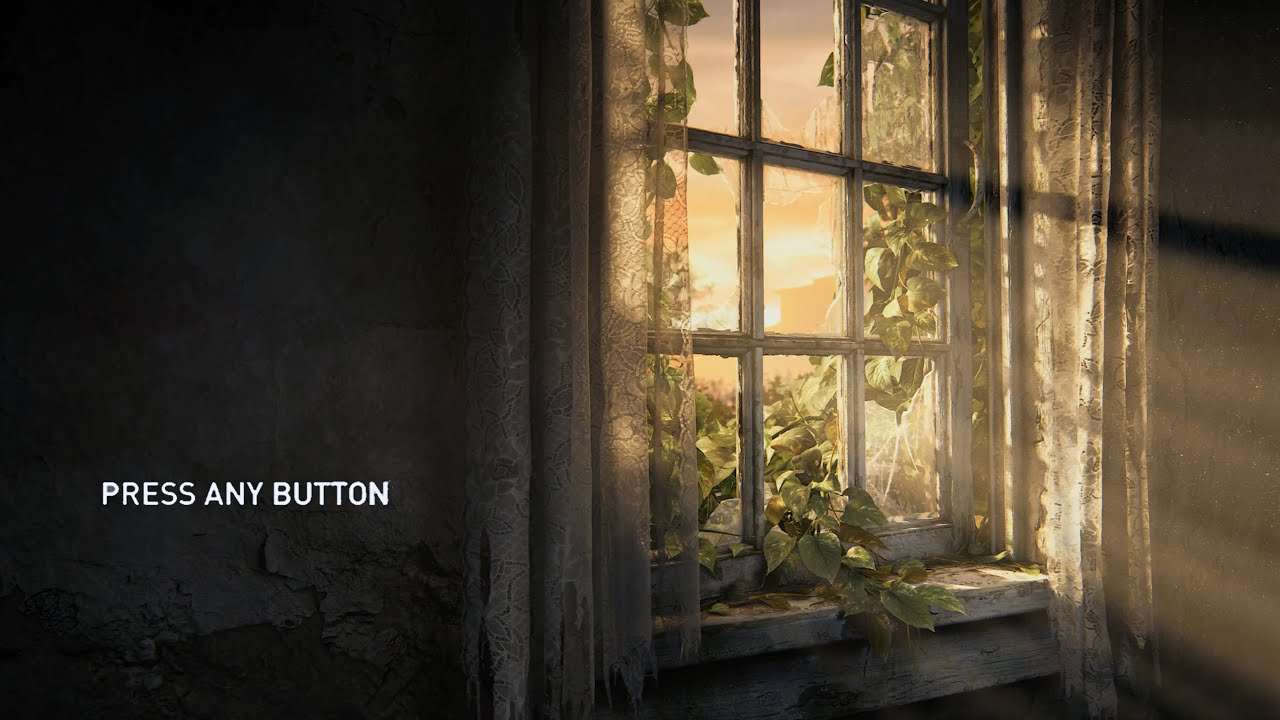
\includegraphics[width=\textwidth]{pages/img/TLOUMenu.jpg}
        \caption{Menú de \textit{The Last of Us} (2013).}
        \label{fig:tloumenu}
    \end{subfigure}
    \hfill
    % Subfigura derecha (Menú TLR)
    \begin{subfigure}[b]{0.45\textwidth}
        \centering
        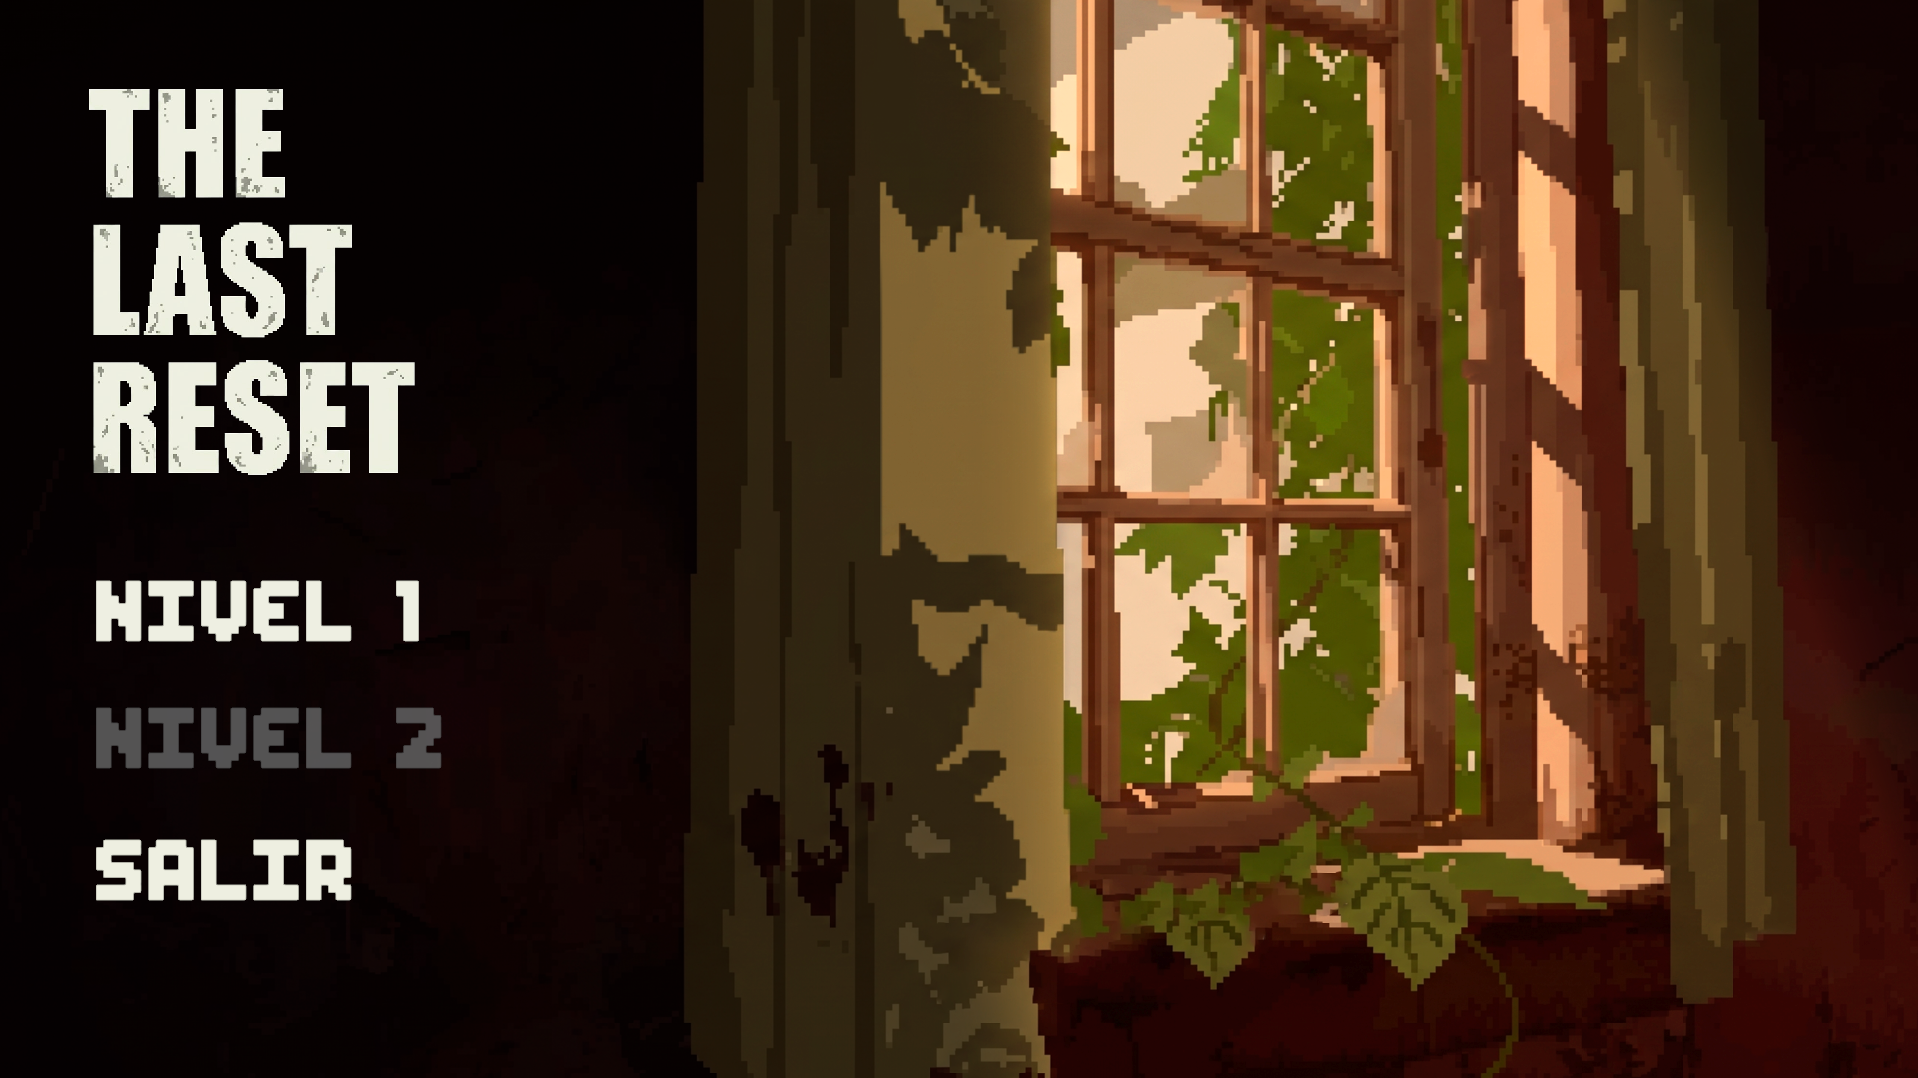
\includegraphics[width=\textwidth]{pages/img/TheLastReset.png}
        \caption{Menú del mundo 1 \textit{The Last Reset}.}
        \label{fig:tlrmenu}
    \end{subfigure}
    \caption{Inspiración del menú de \textit{The Last Reset}.}
    \label{fig:menuTLR}
\end{figure}

Asimismo, la obra integra múltiples referencias y homenajes tanto en su trasfondo narrativo como en la nomenclatura de objetos y personajes. Estas menciones rinden tributo a figuras emblemáticas de los géneros de aventura y \textit{survival horror}, destacando alusiones a personajes icónicos como Joel Miller (de \textit{The Last of Us}) (ver Figura~\ref{fig:joel}) o Leon S. Kennedy (de \textit{Resident Evil}) (ver Figura~\ref{fig:leon}), objetos y armas como el clásico revólver Réquiem de la misma saga \textit{Resident Evil} (ver Figura~\ref{fig:requiem}) y otros múltiples aspectos narrativos. Este recurso no solo enriquece el contexto narrativo, sino que refuerza la identidad del proyecto como un homenaje directo a las influencias que inspiraron su desarrollo.

\begin{figure}[htbp]
    \centering
    % Subfigura izquierda (Joel)
    \begin{subfigure}[b]{0.26\textwidth}
        \centering
        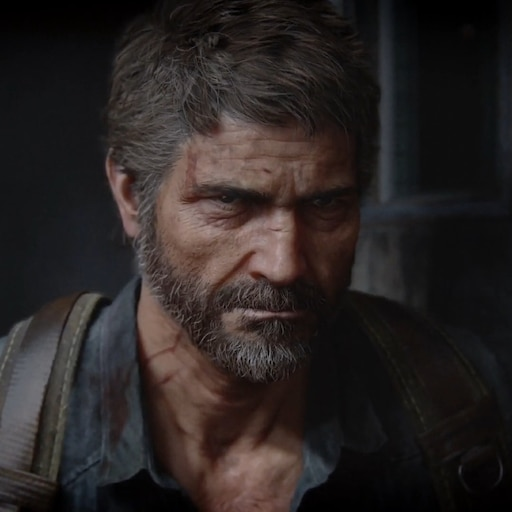
\includegraphics[width=\textwidth]{pages/img/Joel.jpg}
        \caption{Joel Miller de \textit{The Last of Us}.}
        \label{fig:joel}
    \end{subfigure}
    \hfill
    % Subfigura del centro (Leon)
    \begin{subfigure}[b]{0.26\textwidth}
        \centering
        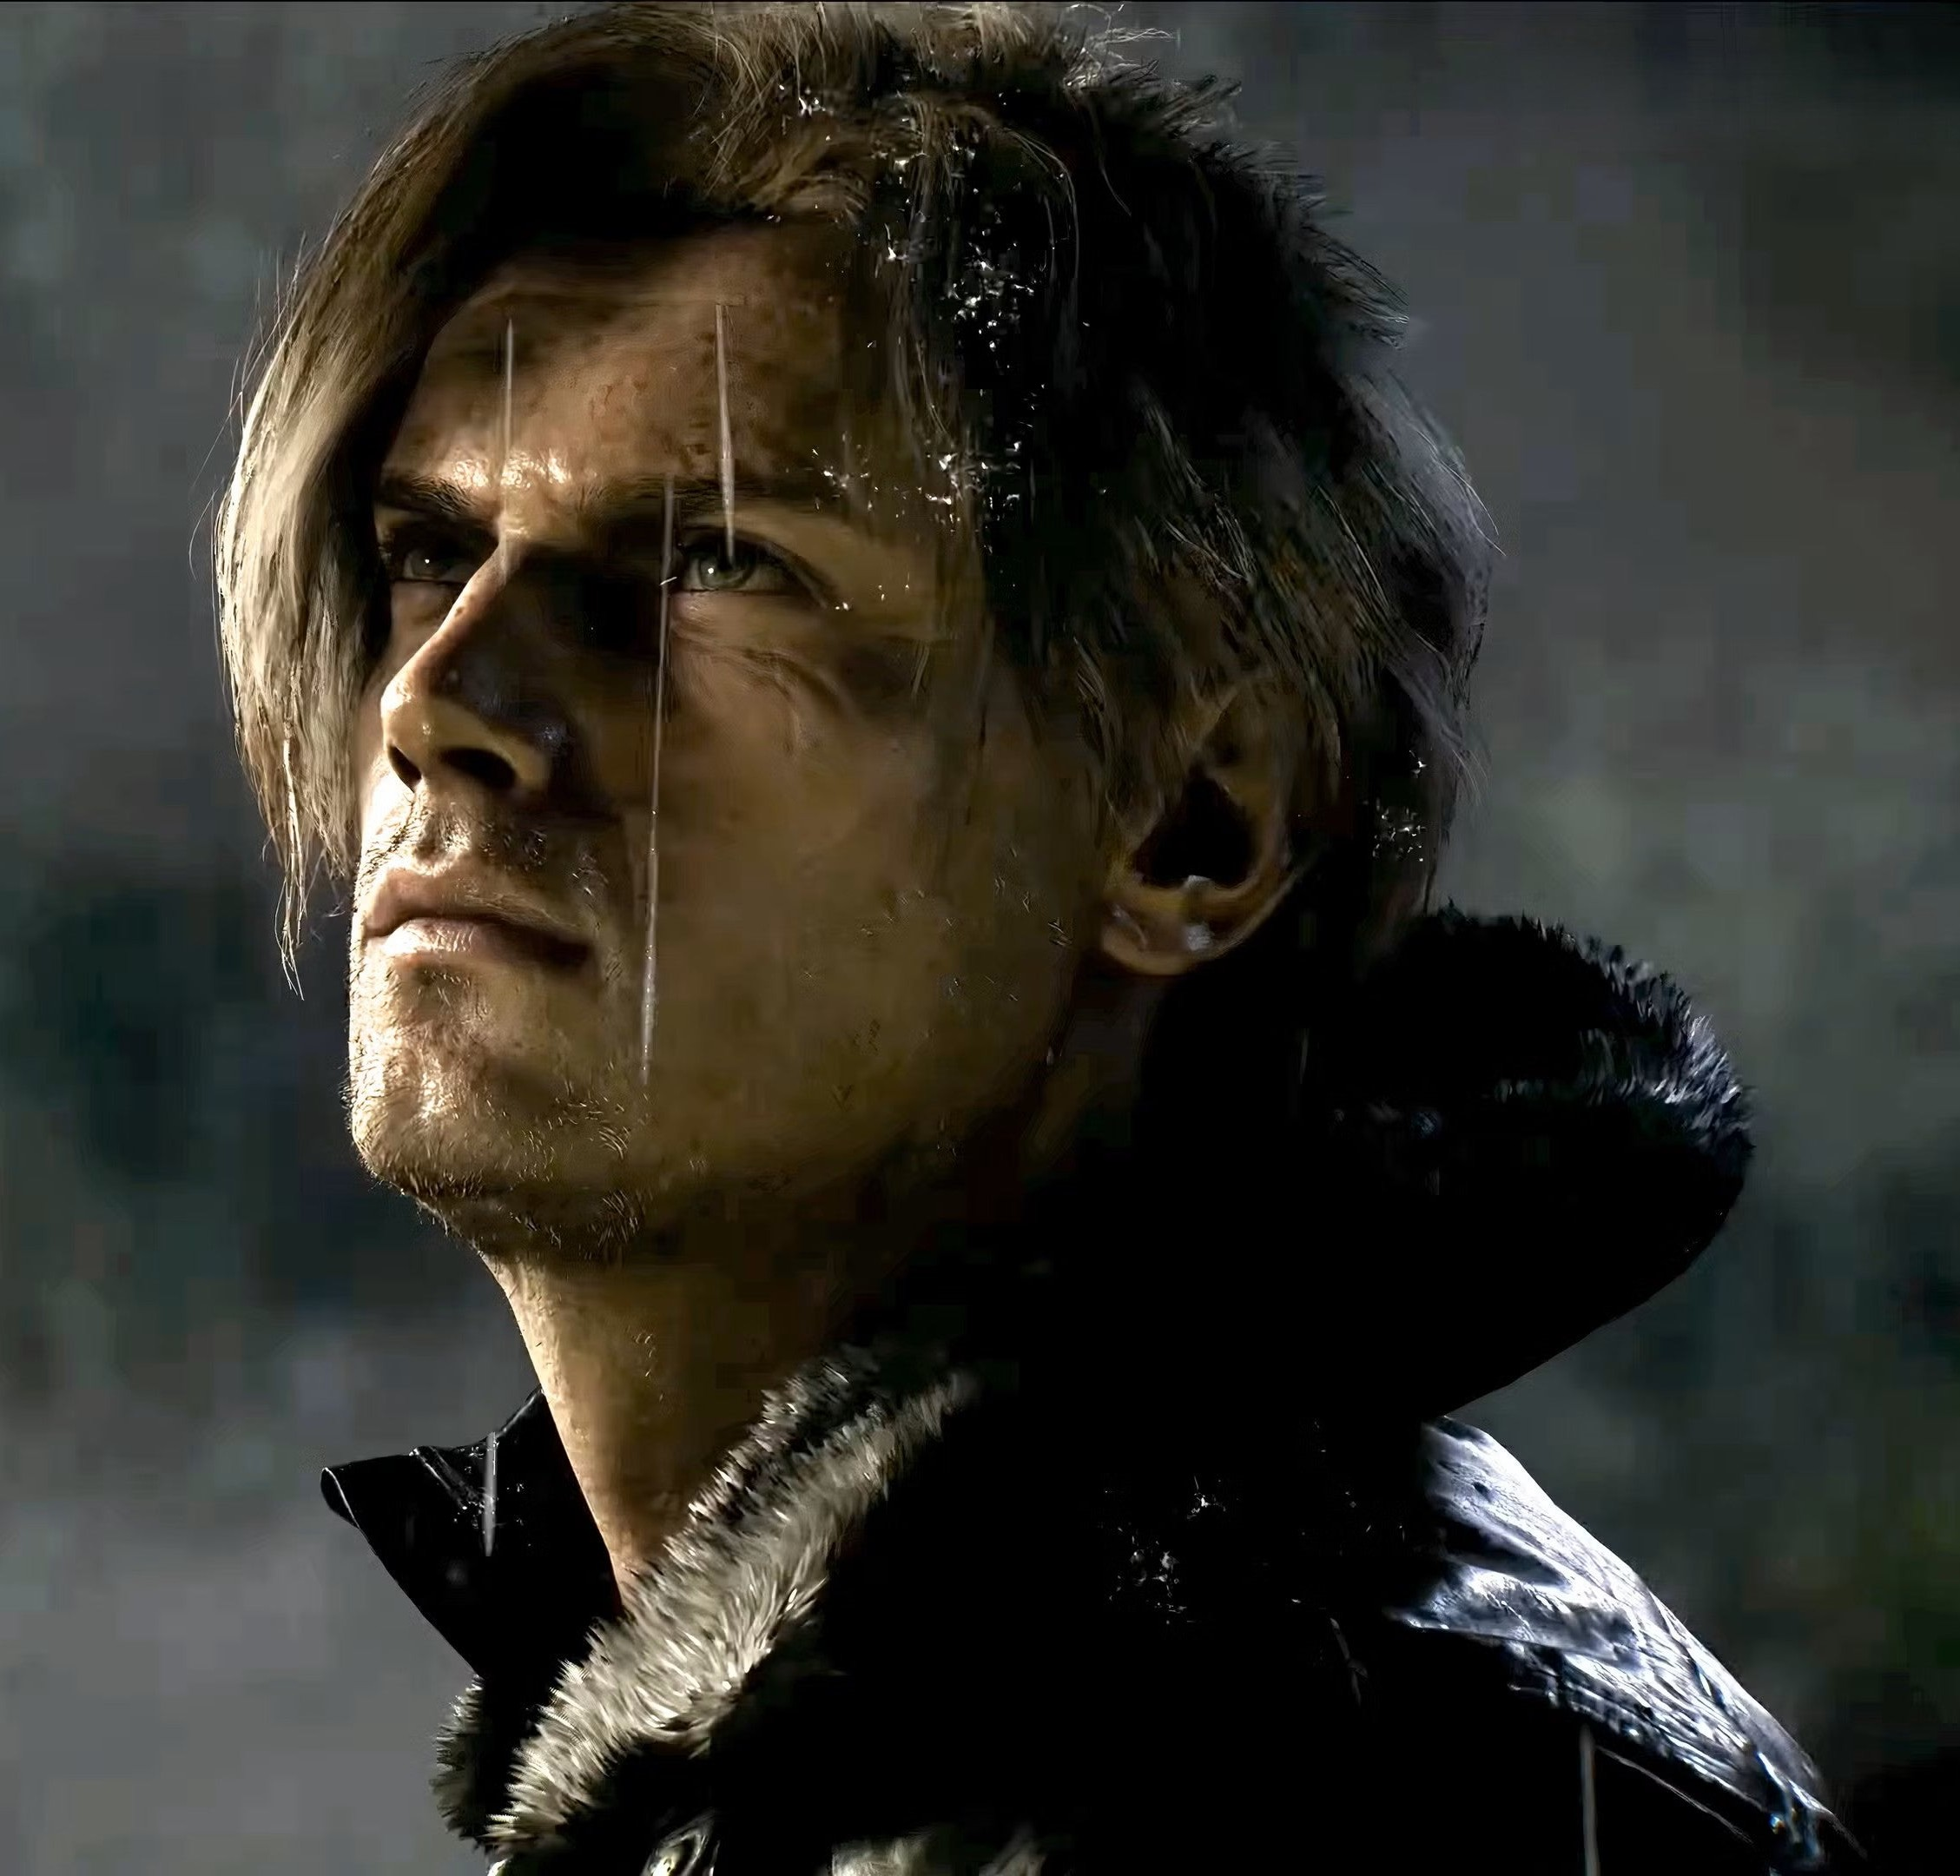
\includegraphics[width=\textwidth]{pages/img/Leon.jpg}
        \caption{Leon S. Kennedy de \textit{Resident Evil}.}
        \label{fig:leon}
    \end{subfigure}
    \hfill
     % Subfigura derecha (Requiem)
    \begin{subfigure}[b]{0.26\textwidth}
        \centering
        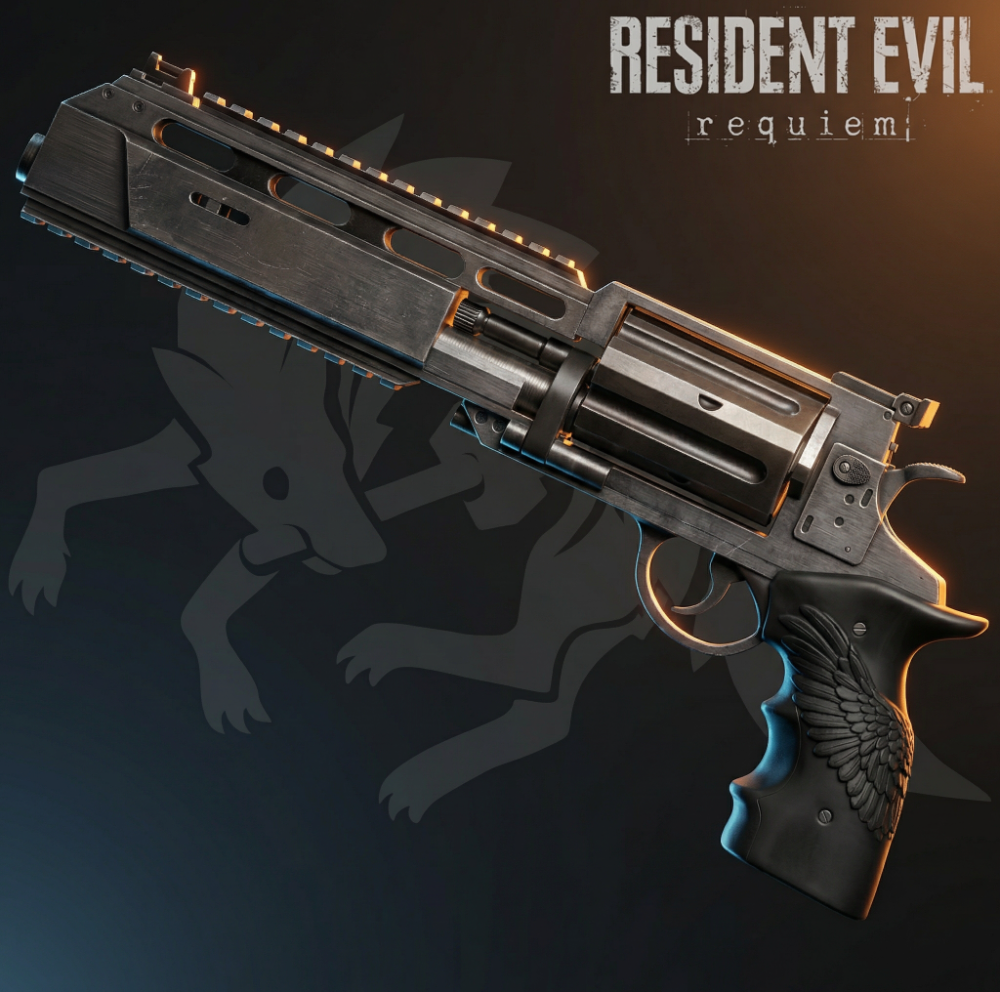
\includegraphics[width=\textwidth]{pages/img/Requiem.png}
        \caption{Revólver Réquiem de \textit{Resident Evil}.}
        \label{fig:requiem}
    \end{subfigure}
    \caption{Inspiraciones de \textit{The Last of Us} y \textit{Resident Evil}.}
    \label{fig:TLOU_RE}
\end{figure}

\subsubsection{Historia y Desarrollo de los Niveles}

\textbf{Nivel 1 (Acción):}
El nivel comienza situando al jugador en mitad de una calle desolada de la ciudad de Boston (E.E.U.U.) (ver Figura~\ref{fig:nivel1}). La consola se encarga de darle las primeras directrices: debe encontrar un gran contenedor rojo para ayudar a ``alguien''. La ambientación nos introduce en un mundo asolado por una epidemia biológica causada por el ``Virus M'', un guiño directo al famoso Virus T de la saga \textit{Resident Evil}. 

En esta primera sección, el jugador debe abrirse paso por las calles derrotando a los infectados mediante un sistema de combate cuerpo a cuerpo. Al llegar al contenedor rojo, el protagonista encuentra a un superviviente. Dado que nuestro protagonista es consciente de que está dentro de un videojuego y conoce las reglas narrativas del medio, se muestra desconfiado y cauteloso con el desconocido, actuando como un personaje más de la simulación para no levantar sospechas. El superviviente le explica que las puertas del contenedor están selladas y que la única forma de abrirlas es conseguir tres cajas de herramientas que los militares federales (referencia a FEDRA en \textit{The Last of Us}) han dejado repartidas por las calles del escenario. Una vez que el jugador explora el mapa, recoge las cajas y las lleva de vuelta, las puertas se abren. Al hablar de nuevo con el superviviente, este revela su nombre: Joel (referencia directa a \textit{The Last of Us}). Joel le cuenta que necesita ir al centro de la ciudad para encontrarse con su amigo Leon (referencia directa a \textit{Resident Evil}) y, aunque nuestro protagonista no termina de fiarse de él, decide aceptar y marchar a su lado.

\begin{figure}[htbp]
    \centering
    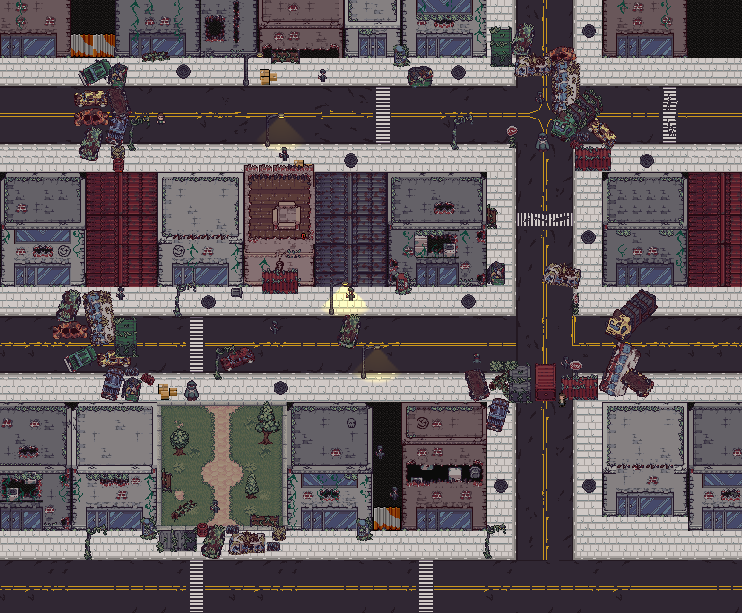
\includegraphics[width=0.7\textwidth]{pages/img/Nivel1.png}
    \caption{Vista general del Nivel 1 de \textit{The Last Reset}.}
    \label{fig:nivel1}
\end{figure}

\textbf{Nivel 2 (Supervivencia):}
El segundo nivel nos traslada al centro de la ciudad (ver Figura~\ref{fig:nivel2}), pero con un imprevisto: el protagonista ha llegado al punto de encuentro solo, ya que Joel se ha desviado para ir a buscar a una niña pequeña (otra alusión directa a la trama de \textit{The Last of Us}). Durante su exploración por el escenario, el protagonista encuentra una pistola abandonada con las iniciales ``L.S.K.'' grabadas en su culata, cuya descripción en el inventario la define como una ``Réquiem'' (un guiño al arma clásica de la saga \textit{Resident Evil}).

Armado con la pistola, el protagonista debe explorar el mapa (compuesto por calles, oficinas y un parque) enfrentándose a nuevos tipos de infectados y buscando pistas. Por el escenario se encuentran repartidas una serie de notas a modo de diario escritas por un tal ``L.S.K.'' (Leon S. Kennedy). A través de ellas, el jugador descubre la historia de Leon: llegó al punto de encuentro y esperó durante días a Joel, pero fue mordido por un infectado el primer día. Las notas narran el avance de la infección irreversible del Virus M y cómo Leon intentó esconderse de los zombies y de los militares federales en las oficinas donde trabajaba (ver Figura~\ref{fig:nivel2.1}). El diario da a entender su trágico final: Leon murió solo y se convirtió en zombie dentro de la oficina que usaba como refugio (la misma oficina donde el jugador se encuentra a un zombie específico junto a una cama). 

En sus escritos, Leon menciona que hay un coche disponible para escapar, pero que lo ha bloqueado con un teclado digital para que nadie lo use antes de que llegue Joel. El código es una fecha muy importante para él: su cumpleaños, la cual coincide con la fecha en la que se sugiere que murió convertido en zombie. El protagonista debe descifrar este código uniendo los cabos sueltos de las notas, introducir la contraseña en el coche y arrancar el motor para huir del lugar, completando así el segundo nivel y logrando superar el primer mundo de \textit{Reset}.

\begin{figure}[htbp]
    \centering
    \begin{subfigure}[b]{0.49\textwidth}
        \centering
        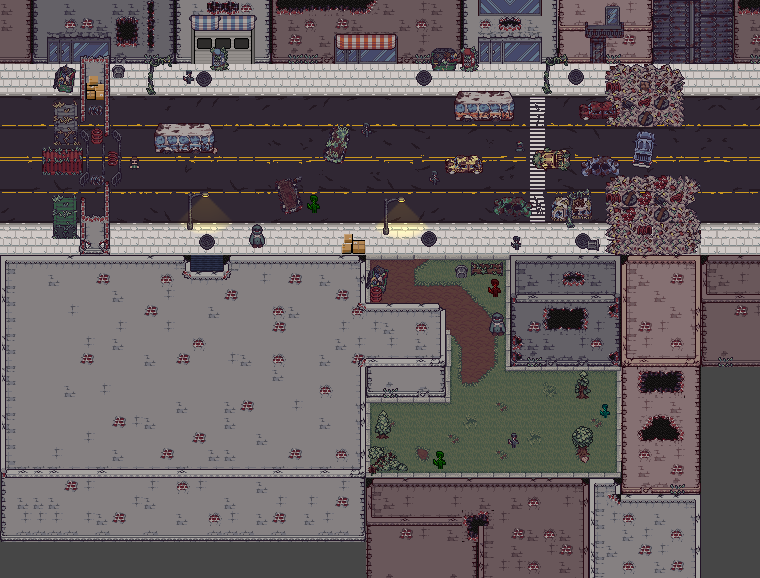
\includegraphics[width=\textwidth]{pages/img/Nivel2.png}
        \caption{Calle central.}
        \label{fig:nivel2}
    \end{subfigure}
    \hfill
    \begin{subfigure}[b]{0.49\textwidth}
        \centering
        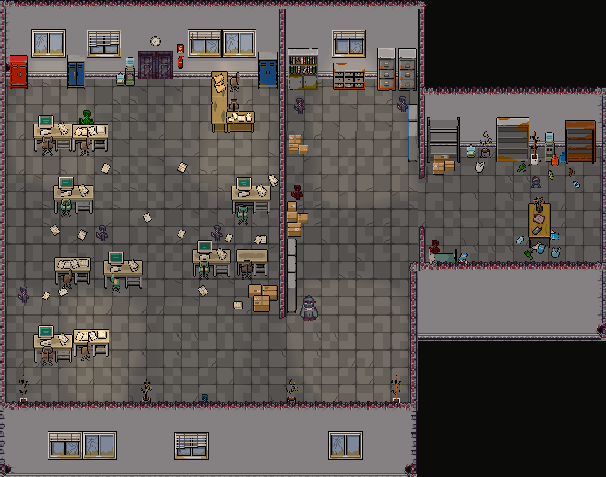
\includegraphics[width=\textwidth]{pages/img/Nivel2.1.png}
        \caption{Oficinas.}
        \label{fig:nivel2.1}
    \end{subfigure}
    \caption{Nivel 2 de \textit{The Last Reset}.}
    \label{fig:Mundo1_Nivel2}
\end{figure}

% =========================================================================
\subsection{Mundo 2: Entorno de Plataformas Vectoriales (``Super Reset Bros'')}
\label{subsec:mundo2}

\subsubsection{Inspiración y Estética}
La inspiración básica para este segundo mundo proviene del juego que, sin duda alguna, redefinió la industria y se consolidó como el referente absoluto del género de plataformas. Titulado en el proyecto como ``Super Reset Bros'', este entorno rinde un tributo directo a la mítica saga japonesa \textit{Super Mario Bros} (ver Figura~\ref{fig:refeSRB}). Dicha franquicia representa el punto de inflexión donde los videojuegos comenzaron a evolucionar desde su etapa más arcade hacia títulos con mayor trasfondo, coherencia visual y diseño de mundos, todo ello estructurado sobre una base jugable tan aparentemente simple como el salto.

\begin{figure}[htbp]
    \centering
    \begin{subfigure}[b]{0.45\textwidth}
        \centering
        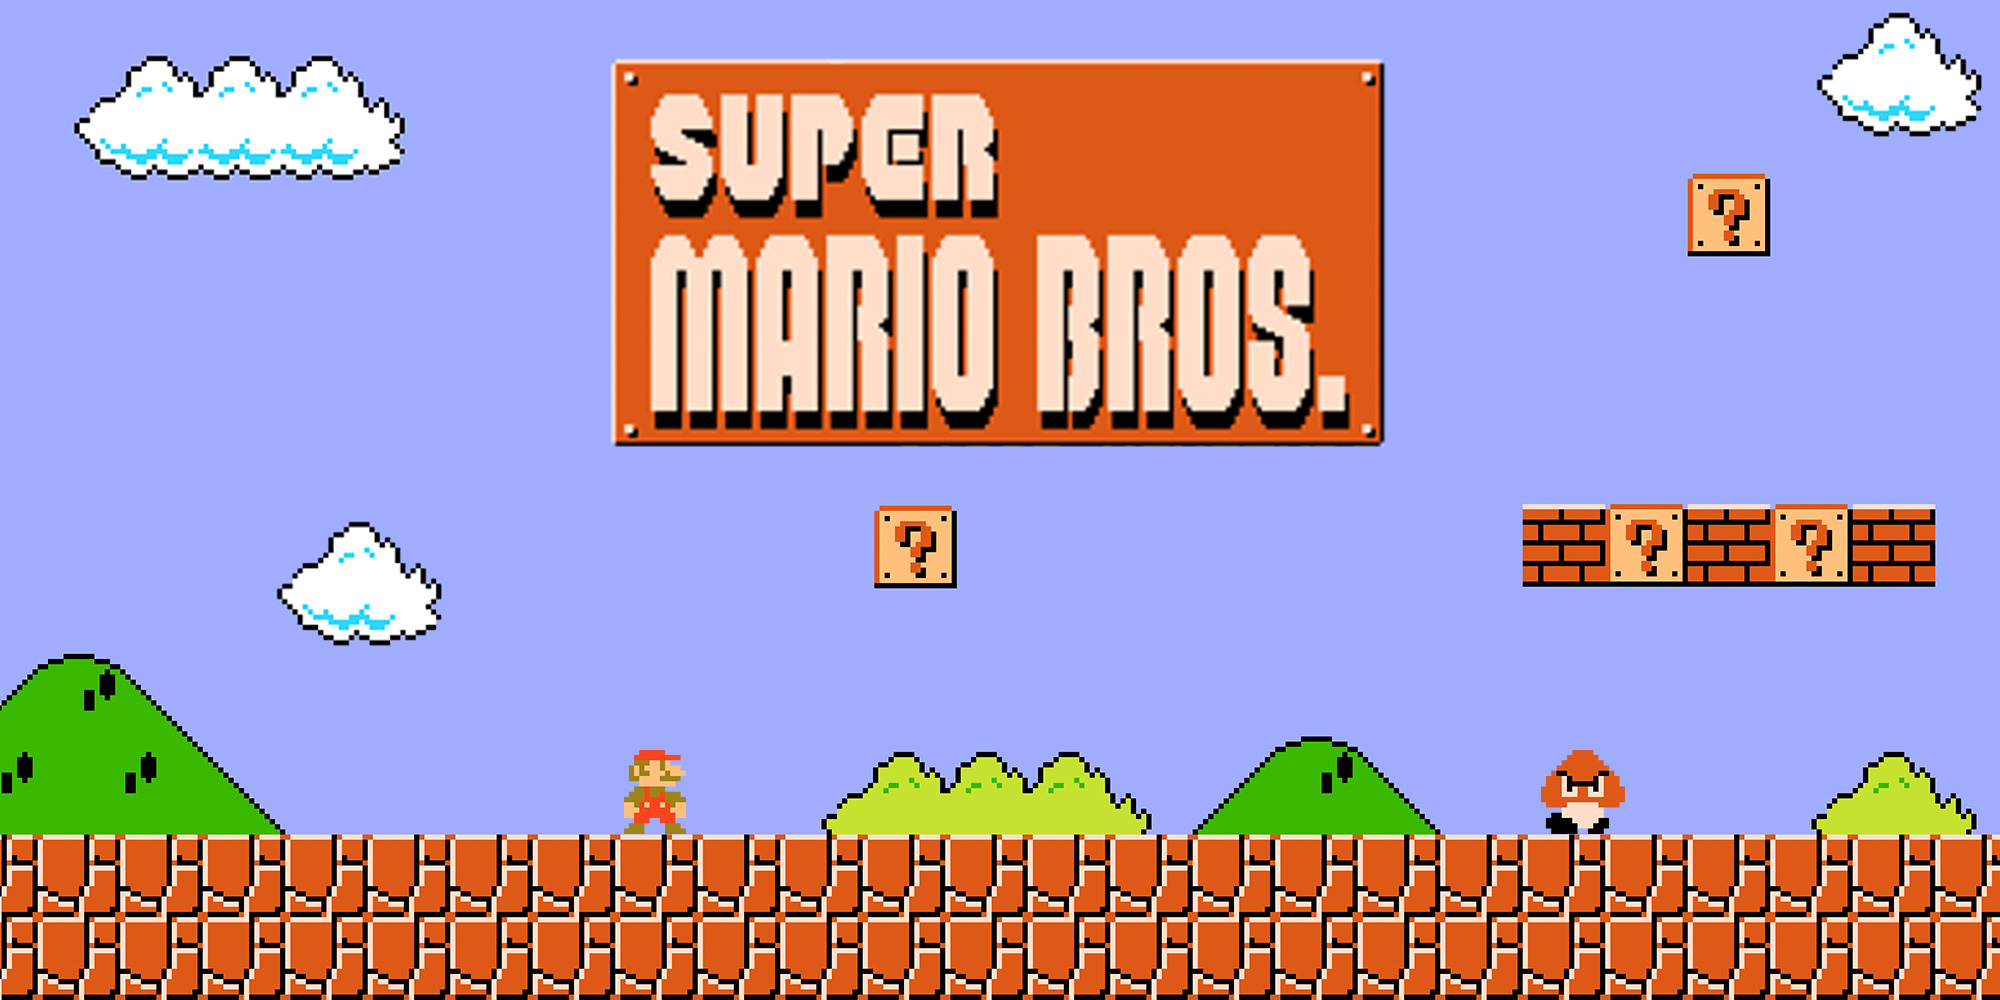
\includegraphics[width=\textwidth]{pages/img/MarioBros.jpg}
        \caption{Menú de \textit{Super Mario Bros} (1985).}
        \label{fig:mario_menu}
    \end{subfigure}
    \hfill
    \begin{subfigure}[b]{0.45\textwidth}
        \centering
        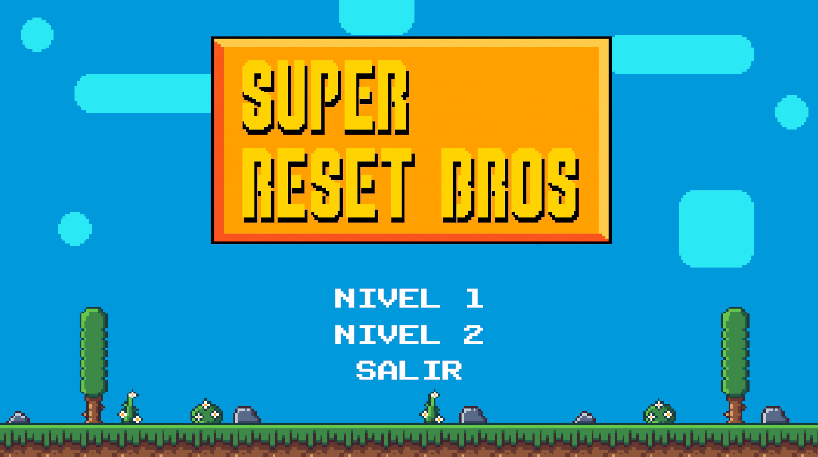
\includegraphics[width=\textwidth]{pages/img/SuperResetBros.png}
        \caption{Menú de \textit{Super Reset Bros}.}
        \label{fig:srb_menu}
    \end{subfigure}
    \caption{Inspiración de \textit{Super Reset Bros}.}
    \label{fig:refeSRB}
\end{figure}

Para el primer nivel, se busca recrear esa esencia clásica mediante bloques de ladrillo, plataformas flotantes y enemigos que patrullan el escenario con comportamientos diversos (tales como patrullas básicas, saltos, lanzamientos de proyectiles, disparos o rebotes), haciendo alusión directa a los antagonistas más míticos de la franquicia. Sin embargo, de cara al segundo nivel, se plantea un giro radical al subgénero de las plataformas. La intención principal es enfocar la jugabilidad hacia el plataformeo de precisión y la dificultad exponencial, un estilo muy demandado por el perfil de jugador actual que busca retos exigentes y la superación de desafíos complejos.

Para lograr esto sin romper la cohesión del juego, se mantiene la misma estética pixel art inspirada en \textit{Super Mario Bros} (garantizando así la coherencia visual de todo el mundo), pero integrando en su diseño el núcleo mecánico y la filosofía de títulos modernos como \textit{Celeste} o \textit{Super Meat Boy}. En estas obras, la habilidad del jugador, el diseño milimétrico de los obstáculos y la inercia del movimiento toman todo el protagonismo. Esto permite crear una experiencia jugable muy superior mecánicamente, donde el jugador debe exprimir al máximo los mismos controles básicos de movimiento y salto que ya dominaba en el nivel anterior, pero aplicándolos ahora a situaciones de precisión extrema y coordinación espacial.

\subsubsection{Historia y Desarrollo de los Niveles}
En consonancia con sus referentes clásicos, la narrativa de este segundo mundo hace alusión directa a los primeros títulos de la saga \textit{Super Mario}, donde la exposición textual era mínima y el contexto argumental se vinculaba de forma directa a la propia representación visual y al entorno del nivel. En este sector, el escenario plantea una dimensión prehistórica digital, un entorno poblado por enemigos inspirados en dinosaurios y criaturas derivadas de fósiles.

La progresión física del escenario guía al protagonista a través de un viaje horizontal y vertical muy marcado en el primer nivel. El recorrido se inicia atravesando el ``Valle de los Dinosaurios'' (ver Figura~\ref{fig:nmundo2.1}) mediante una jugabilidad de desplazamiento lateral clásico (\textit{side-scrolling}). Posteriormente, para acceder al portal de salida, el jugador debe adentrarse en el interior de una montaña que actúa como torre de ascenso hacia el ``Reino de los Cielos'', implementando mecánicas de desplazamiento vertical ascendente (\textit{up-scrolling}) que homenajean a los niveles de torre de la saga de Nintendo.

\begin{figure}[htbp]
    \centering
    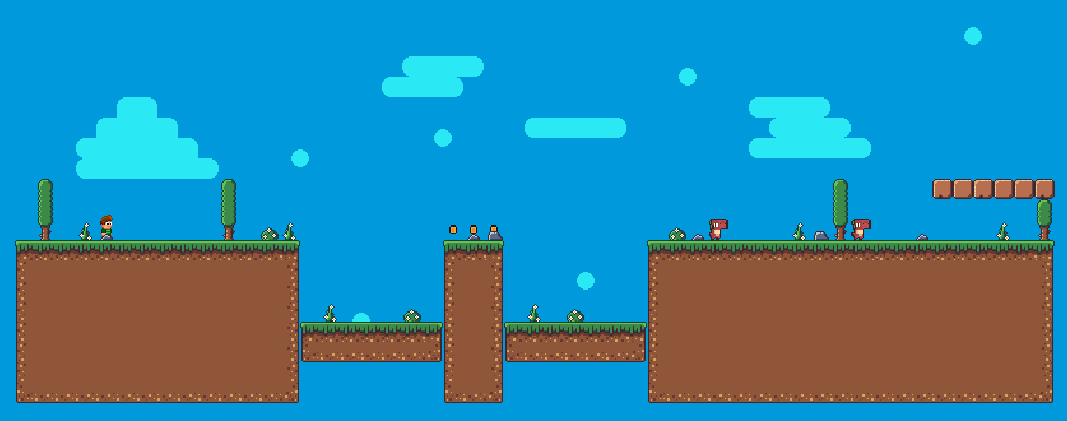
\includegraphics[width=0.75\textwidth]{pages/img/Mundo2.1.png}
    \caption{Inicio del Nivel 1 de \textit{Super Reset Bros}.}
    \label{fig:mundo2.1}
\end{figure}

Dado que la trama explícita del nivel es deliberadamente minimalista para respetar la estética retro, este espacio se aprovecha en los diálogos que se producen tanto en los niveles como en el Hub entre niveles para desarrollar la evolución del protagonista y su interacción con la consola. A través de estas conversaciones en el Nexo, se aprecia una conformidad creciente en la actitud del protagonista respecto a su misión. La relación inicial, caracterizada por la rigidez de un sistema directivo y el miedo de un aprendiz desubicado, comienza a transformarse de forma paulatina en un vínculo de confianza mutua más consolidado. A lo largo de esta transición, el protagonista comienza a manifestar, de manera muy gradual, una mayor determinación, iniciativa y valentía ante los fallos del sistema.

De este modo, en el segundo nivel de este mundo (ver Figura~\ref{fig:mundo2.2}), el contexto narrativo se reduce al mínimo con el fin de priorizar el plano puramente mecánico. Esta ausencia intencionada de carga argumental permite que la atención del jugador se concentre por completo en asimilar y superar el exigente reto de precisión que plantea la cueva en la que despierta el personaje al cruzar el portal. Una vez completado este segundo nivel, se desencadena el diálogo final de la demo en el Hub. En esta conversación, la consola y el protagonista comienzan a profundizar en la verdadera razón por la cual el sistema eligió a este personaje específico del tutorial como protagonista. Sin embargo, esta revelación es interrumpida abruptamente por la intrusión del villano —cuya identidad aún permanece oculta— en la base de la memoria del sistema, provocando un apagado instantáneo precedido por una cuenta atrás de diez segundos. La demo concluye de forma repentina con un fundido a negro a mitad de dicha cuenta regresiva, dejando la resolución del conflicto en suspense de cara a futuros desarrollos.

\begin{figure}[htbp]
    \centering
    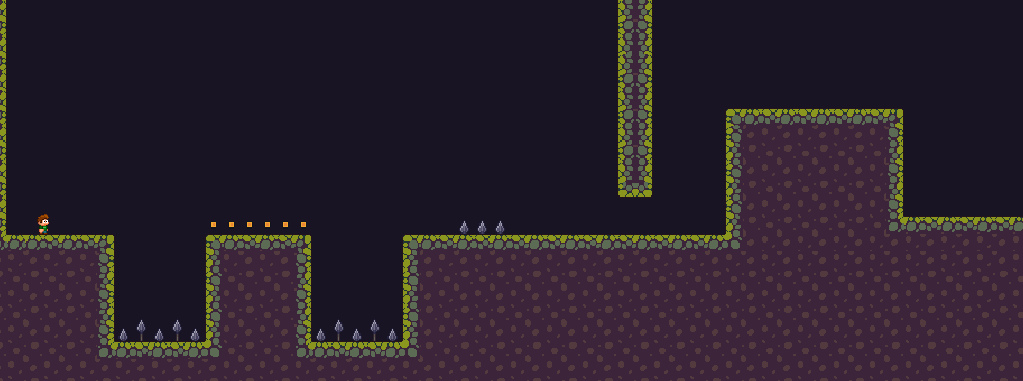
\includegraphics[width=0.75\textwidth]{pages/img/Mundo2.2.png}
    \caption{Inicio del Nivel 2 de \textit{Super Reset Bros}.}
    \label{fig:mundo2.2}
\end{figure}
% =========================================================================
% =========================================================================
\section{Mecánicas y Dinámicas de Juego}
\label{sec:mecanicas_dinamicas_detallado}

En esta sección se analiza de forma simplificada el comportamiento interactivo del juego desde la perspectiva de las mecánicas (los controles de entrada o \textit{inputs} del jugador y las reglas del software) y las dinámicas (el comportamiento en tiempo de ejecución resultante de la interacción del usuario con las mecánicas). El diseño está estructurado de manera que la complejidad mecánica aumente de forma progresiva a lo largo de cada mundo.

% =========================================================================
\subsection{Mundo 1: Supervivencia Cenital (``The Last Reset'')}
\label{subsec:mecanicas_mundo1}

Este mundo introduce una jugabilidad en perspectiva cenital (\textit{Top-Down}) centrada en el movimiento libre bidimensional, la gestión de inventario y el combate táctico.

\subsubsection{Nivel 1 (Acción)} (ver Figura~\ref{fig:controles1})
\begin{itemize}
    \item \textbf{Mecánicas del Jugador:}
    \begin{itemize}
        \item \textit{Movimiento Bidimensional:} Control de ejes cartesianos implementado mediante las teclas \texttt{W} (arriba), \texttt{A} (izquierda), \texttt{S} (abajo) y \texttt{D} (derecha).
        \item \textit{Esquiva (Dash):} Desplazamiento rápido de corta duración en la dirección del movimiento pulsando la tecla \texttt{Espacio} (\textit{Space}).
        \item \textit{Ataque Cuerpo a Cuerpo:} Golpe físico básico direccionado mediante el apuntado de la cámara, activado mediante el \texttt{Clic Izquierdo} del ratón.
        \item \textit{Interacción:} Activación de diálogos e interruptores del mapa con la tecla \texttt{E}.
        \item \textit{Gestión de Salud:} Pausa de la acción y apertura de la interfaz de inventario mediante la tecla \textit{P}. O selección \textit{in game} rápida del tipo de consumible médico con la tecla \textit{Tab} y aplicación de la curación activa mediante la tecla \textit{Q}.
    \end{itemize}
    
    \item \textbf{Dinámicas de Juego:}
    El nivel se enfoca en la exploración y la familiarización del usuario con el combate cuerpo a cuerpo. La dinámica de progresión requiere que el jugador explore de manera no lineal calles desoladas en busca de recursos (suministros médicos) y derrote patrullas enemigas. Para desbloquear el contenedor rojo de salida que obstruye el camino, el jugador debe explorar el nivel hasta localizar tres cajas de herramientas militares distribuidas en el escenario, las cuales funcionan como llaves lógicas para el sistema de seguridad.
\end{itemize}

\subsubsection{Nivel 2 (Supervivencia)} (ver Figura~\ref{fig:controles1})
\begin{itemize}
    \item \textbf{Mecánicas del Jugador:}
    El principal enfoque del nivel anterior consistía en familiarizar al jugador con el combate cuerpo a cuerpo, haciendo énfasis en el género \textit{Hack and Slash} para poder avanzar a este segundo nivel con las mecánicas básicas controladas, pudiendo así aumentar la dificultad e introducir nuevas mecánicas y enemigos como el combate a distancia mediante arma de fuego, por ello se añaden:
    \begin{itemize}
        \item \textit{Combate a Distancia (Disparo):} Apuntado libre en 360 grados y disparo proyectil en la dirección del cursor mediante el \texttt{Clic Izquierdo} del ratón.
        \item \textit{Cambio de Arma:} Alternancia instantánea entre el modo cuerpo a cuerpo y el arma a distancia (pistola) mediante el \texttt{Clic Derecho} del ratón.
        \item \textit{Recarga:} Alimentación del cargador activo de la pistola mediante la tecla \texttt{R}, lo que descuenta munición de las ranuras de inventario.
    \end{itemize}
    
    \item \textbf{Dinámicas de Juego:}
    El bucle de juego evoluciona hacia una experiencia de supervivencia opresiva. Los suministros son escasos, obligando a explorar detalladamente oficinas y zonas ocultas para saquear cajas destructibles en busca de vendas y cartuchos de munición. La progresión lógica del nivel está bloqueada por una contraseña de seguridad de cuatro dígitos. La dinámica para resolver este puzle obliga al jugador a buscar y leer cronológicamente diarios en formato de notas olvidadas. La lectura atenta permite al jugador deducir que la clave numérica corresponde a la fecha de cumpleaños de un personaje fallecido, descifrando el enigma para arrancar el coche de escape.
\end{itemize}

\begin{figure}[htbp]
    \centering
    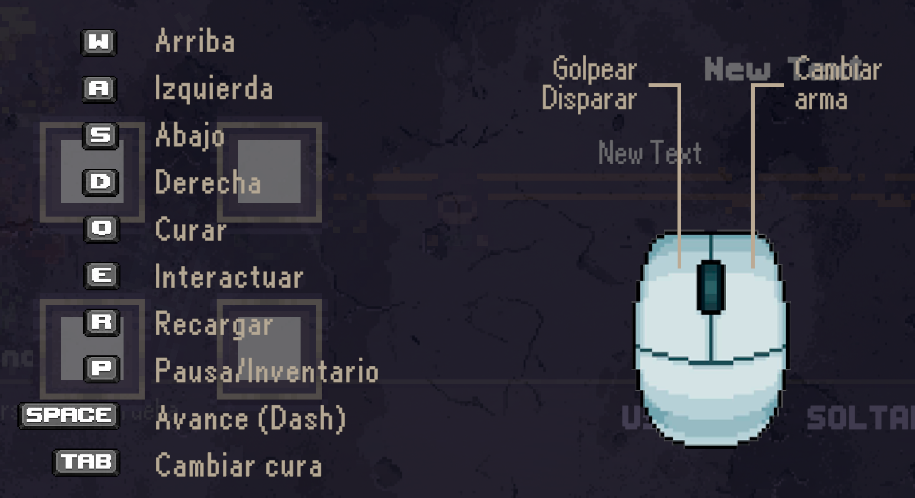
\includegraphics[width=0.5\textwidth]{pages/img/ControlesMundo1.png}
    \caption{Controles globales de \textit{The Last Reset}.}
    \label{fig:controles1}
\end{figure}

% =========================================================================
\subsection{Mundo 2: Plataformas Vectoriales (``Super Reset Bros'')}
\label{subsec:mecanicas_mundo2}

Este mundo transiciona la perspectiva al plano bidimensional lateral (\textit{Side-Scroller}) donde las fuerzas gravitatorias y la inercia aérea definen los desafíos físicos.

\subsubsection{Nivel 1 (Plataformas Clásico)} (ver Figura~\ref{fig:controles2.1})
\begin{itemize}
    \item \textbf{Mecánicas del Jugador:}
    El mapa de control se reduce a la mínima expresión del género de plataformas:
    \begin{itemize}
        \item \textit{Desplazamiento Horizontal:} Movimiento lateral implementado en el eje horizontal mediante las teclas \texttt{A} (izquierda) y \texttt{D} (derecha).
        \item \textit{Salto Básico:} Impulso vertical en contra de la gravedad mediante la tecla \texttt{Espacio} (\textit{Space}).
    \end{itemize}

\begin{figure}[htbp]
    \centering
    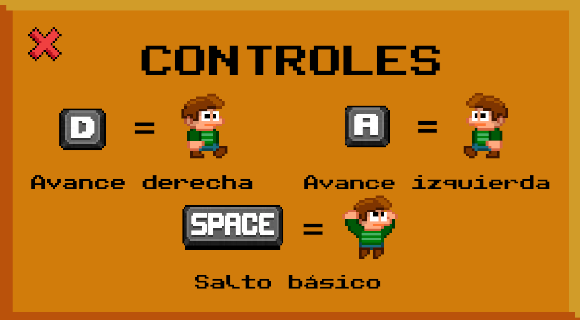
\includegraphics[width=0.5\textwidth]{pages/img/ControlesMundo2.1.png}
    \caption{Controles del Nivel 1 de \textit{Super Reset Bros}.}
    \label{fig:controles2.1}
\end{figure}
    
    \item \textbf{Dinámicas de Juego:}
    El nivel introduce una mecánica de contrarreloj (\textit{Time Attack}) en el que el jugador cuenta con un límite de tiempo decreciente para llegar al portal de salida. La derrota de los enemigos (patrullas clásicas con saltos y disparos de proyectiles) es opcional. El jugador debe optimizar su ritmo de avance y saltos recolectando monedas pequeñas repartidas por el camino principal, las cuales otorgan segundos adicionales, y localizando monedas ocultas (\textit{Dino Cookies}) en zonas secretas que otorgan una bonificación temporal sustancial.
\end{itemize}

\subsubsection{Nivel 2 (Plataformas de Precisión)} (ver Figura~\ref{fig:controles2.1})
\begin{itemize}
    \item \textbf{Mecánicas del Jugador:}
    Se heredan los controles de movimiento básicos horizontales y se desbloquean mecánicas de movilidad avanzada indispensables para la navegación:
    \begin{itemize}
        \item \textit{Doble Salto:} Ejecución de un segundo impulso vertical en el aire mediante una doble pulsación de la tecla \texttt{Espacio} (\texttt{Espacio + Espacio}).
        \item \textit{Salto de Pared (Wall Jump):} Reimpulso vertical en diagonal al realizar un salto colisionando de forma lateral con una pared y pulsando la tecla \texttt{Espacio}.
        \item \textit{Avance Aéreo (Air Dash):} Impulso lineal rápido horizontal en el aire ejecutando la combinación \texttt{Espacio + Shift}.
    \end{itemize}

\begin{figure}[htbp]
    \centering
    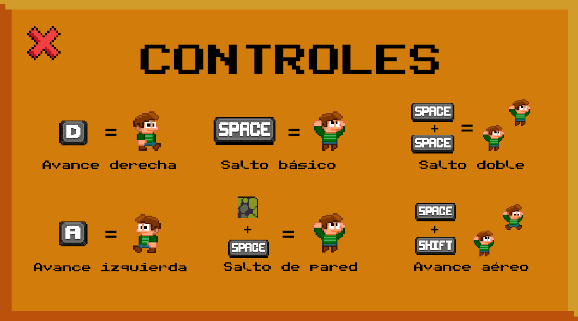
\includegraphics[width=0.5\textwidth]{pages/img/ControlesMundo2.2.png}
    \caption{Controles del Nivel 2 de \textit{Super Reset Bros}.}
    \label{fig:controles2.2}
\end{figure}

    \item \textbf{Dinámicas de Juego:}
    La jugabilidad cambia drásticamente hacia un reto de plataformas de precisión o \textit{parkour} técnico, eliminando por completo la presencia de enemigos. Los escenarios se diseñan como una sucesión de obstáculos letales y fosos de pinchos de muerte instantánea. El jugador experimenta una dinámica de alta concentración basada en el ensayo y error, debiendo encadenar con precisión saltos dobles, rebotes en paredes y avances aéreos para progresar a través de las diferentes plataformas. Para facilitar la navegación aérea, el diseño del nivel incorpora gemas flotantes que restablecen de forma instantánea la capacidad de realizar el avance (\textit{dash}) en el aire. Dado que esta mecánica normalmente requiere que el personaje toque suelo firme para recargarse, la recolección de estas gemas permite superar secciones complejas sin superficies de apoyo, obligando al jugador a mantener un movimiento constante y fluido que exprime al máximo todas las capacidades de movilidad física del avatar.
\end{itemize}